As mentioned in \cref{sec:arkani-hamed-dimop} in the \gls{add} model, the
fundamental scale of the gravitational interaction, $\md$, is brought down to
the electroweak scale ($\md \approx 1~$TeV). At these energies, due to the large
center of mass energy available at \gls{lhc}, the validity of the predictions of
the \gls{eft} become unreliable. For this reason two different sets of limits
have been calculated, one where the full cross section is used and the other
where it is weighted down by a factor $\md^4/\hat{s}^2$ for events where
$\hat{s} > \md^2$, where $\hat{s}$ is the center of mass energy of the
partons~\cite{LEDWeightFactor}.

As an illustration of the problem \cref{fig:shat} shows the $\hat{s}$
distribution in the regions where $250 < \met < 300$~GeV and
$700 < \met < 800$~GeV for the ADD n = 3 and 6 models. The straight line
indicates the excluded $\md$ value before any weighting of the events. This
figure shows that a fraction of the selected events in the signal regions have a
value of $\hat{s}$ that exceeds the limit of validity of the effective field
theory. The general idea of weighting the events is therefore introduced. It
consists in re-evaluating the limit on $\md$ in a conservative way, by
prescribing that all events with $\hat{s}$ exceeding the validity limit should
only weakly contribute to the limit on $\md$. Moreover \cref{fig:shat} shows
that the bulk of the $\hat{s}$ distribution moves towards higher energy values
both in the case when the number of extra dimensions and the $\met$ are
increased. The first case is understood considering the growing of the graviton
mass with the number of extra dimensions showed in \cref{fig:graviton_mass}:
the production of gravitons with higher mass require higher momentum of the
partons. A similar argument holds when the $\met$ is increased, higher values of
missing energy imply the production of heavier gravitons.

\cref{fig:vis_sigma_trunc} shows the visible cross section as a function of the
fundamental Planck scale $\md$ in the $250 < \met < 300$~GeV and
$700 < \met < 800$~GeV regions for the ADD n = 3, 6 models. The solid line is
the visible cross section for all the $\hat{s}$, while in the dashed one a
$\md^4/\hat{s}^2$ weighting factor is applied for events where
$\hat{s} > \md^2$, it can be seen that for $\md = 0$ all events get weighted
down since $\hat{s} > \md^2 = 0$. The black square is the nominal $\md$ value of
the generated sample.
\begin{figure}[!h]
  \centering
  \begin{subfigure}{.48\linewidth}
    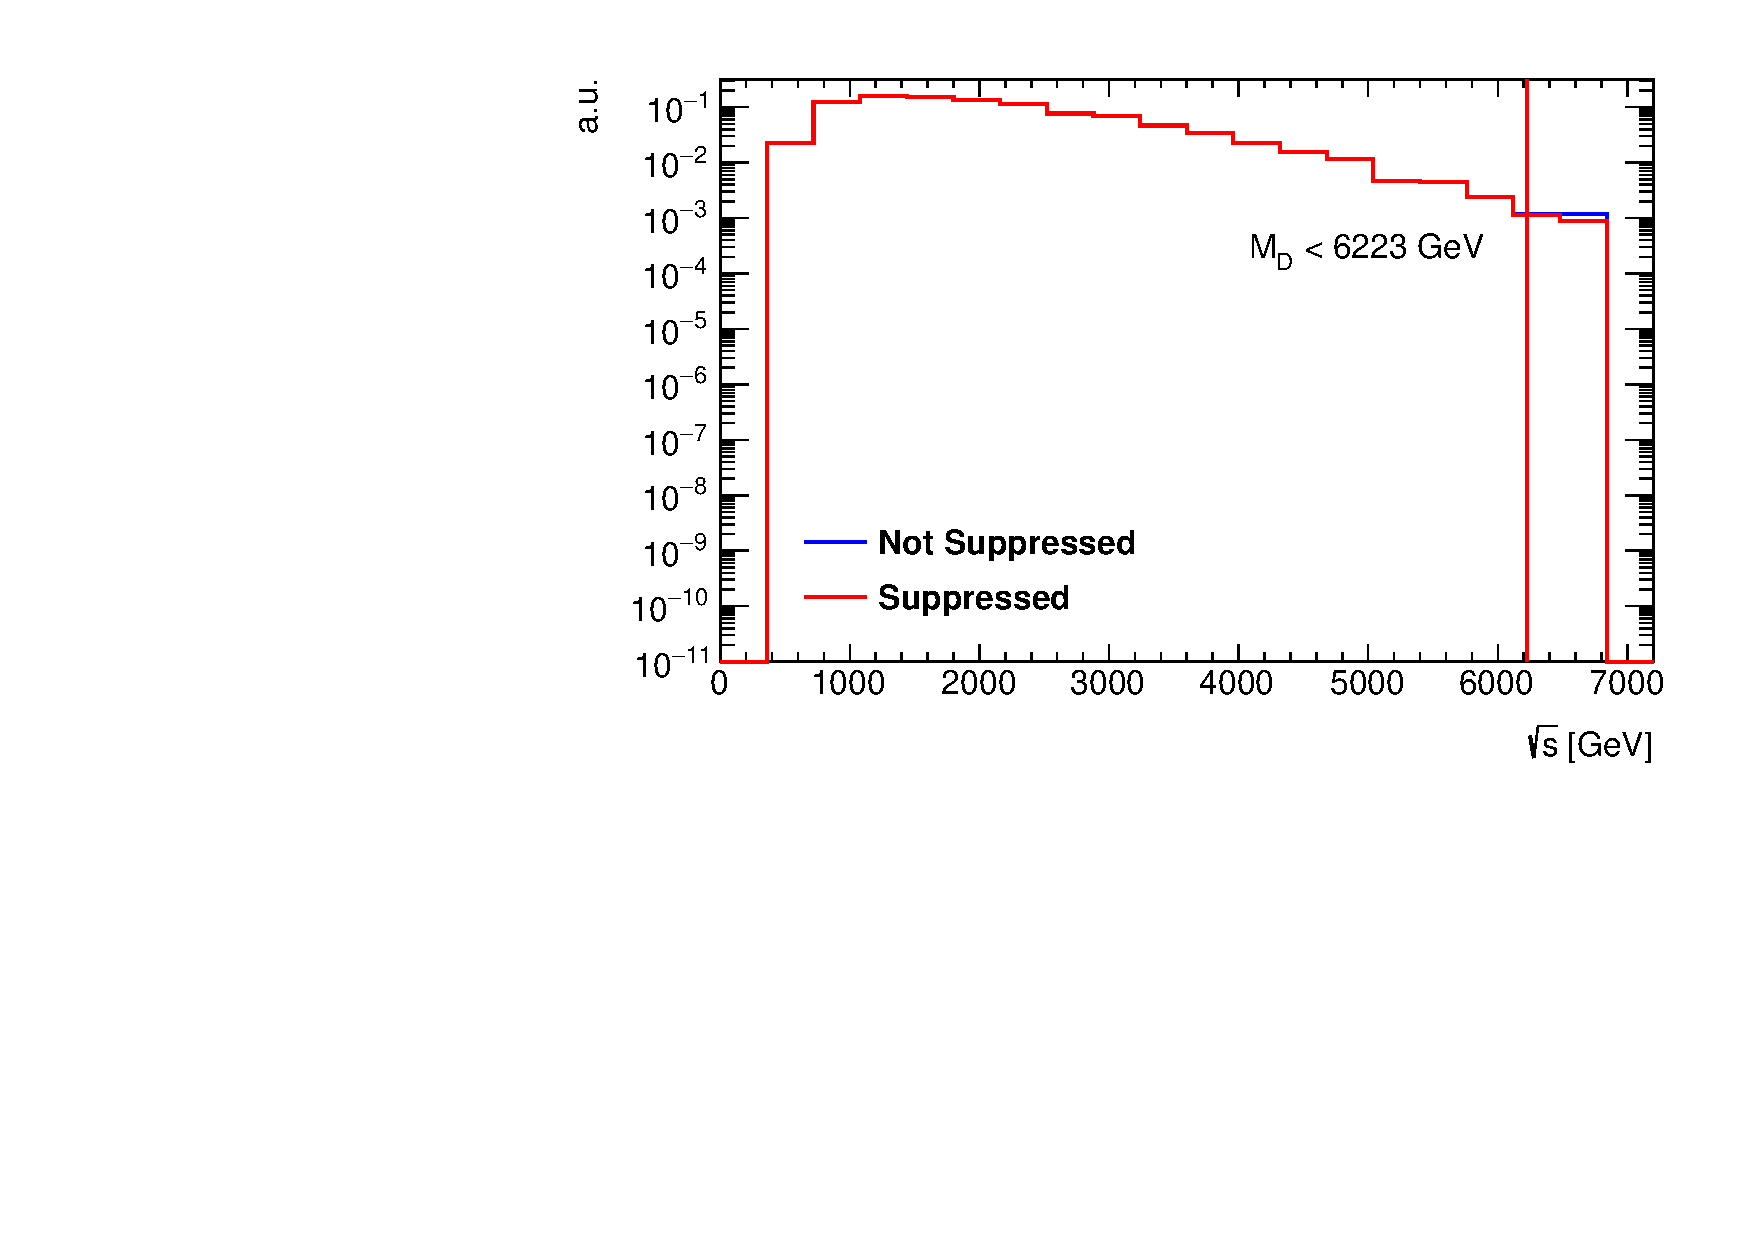
\includegraphics[width=\linewidth]{plot_nD3_SR250}
    \caption{ADD n = 3 for low $\met$ region.}
    \label{fig:shat_n3_250}
  \end{subfigure}
  \begin{subfigure}{.48\linewidth}
    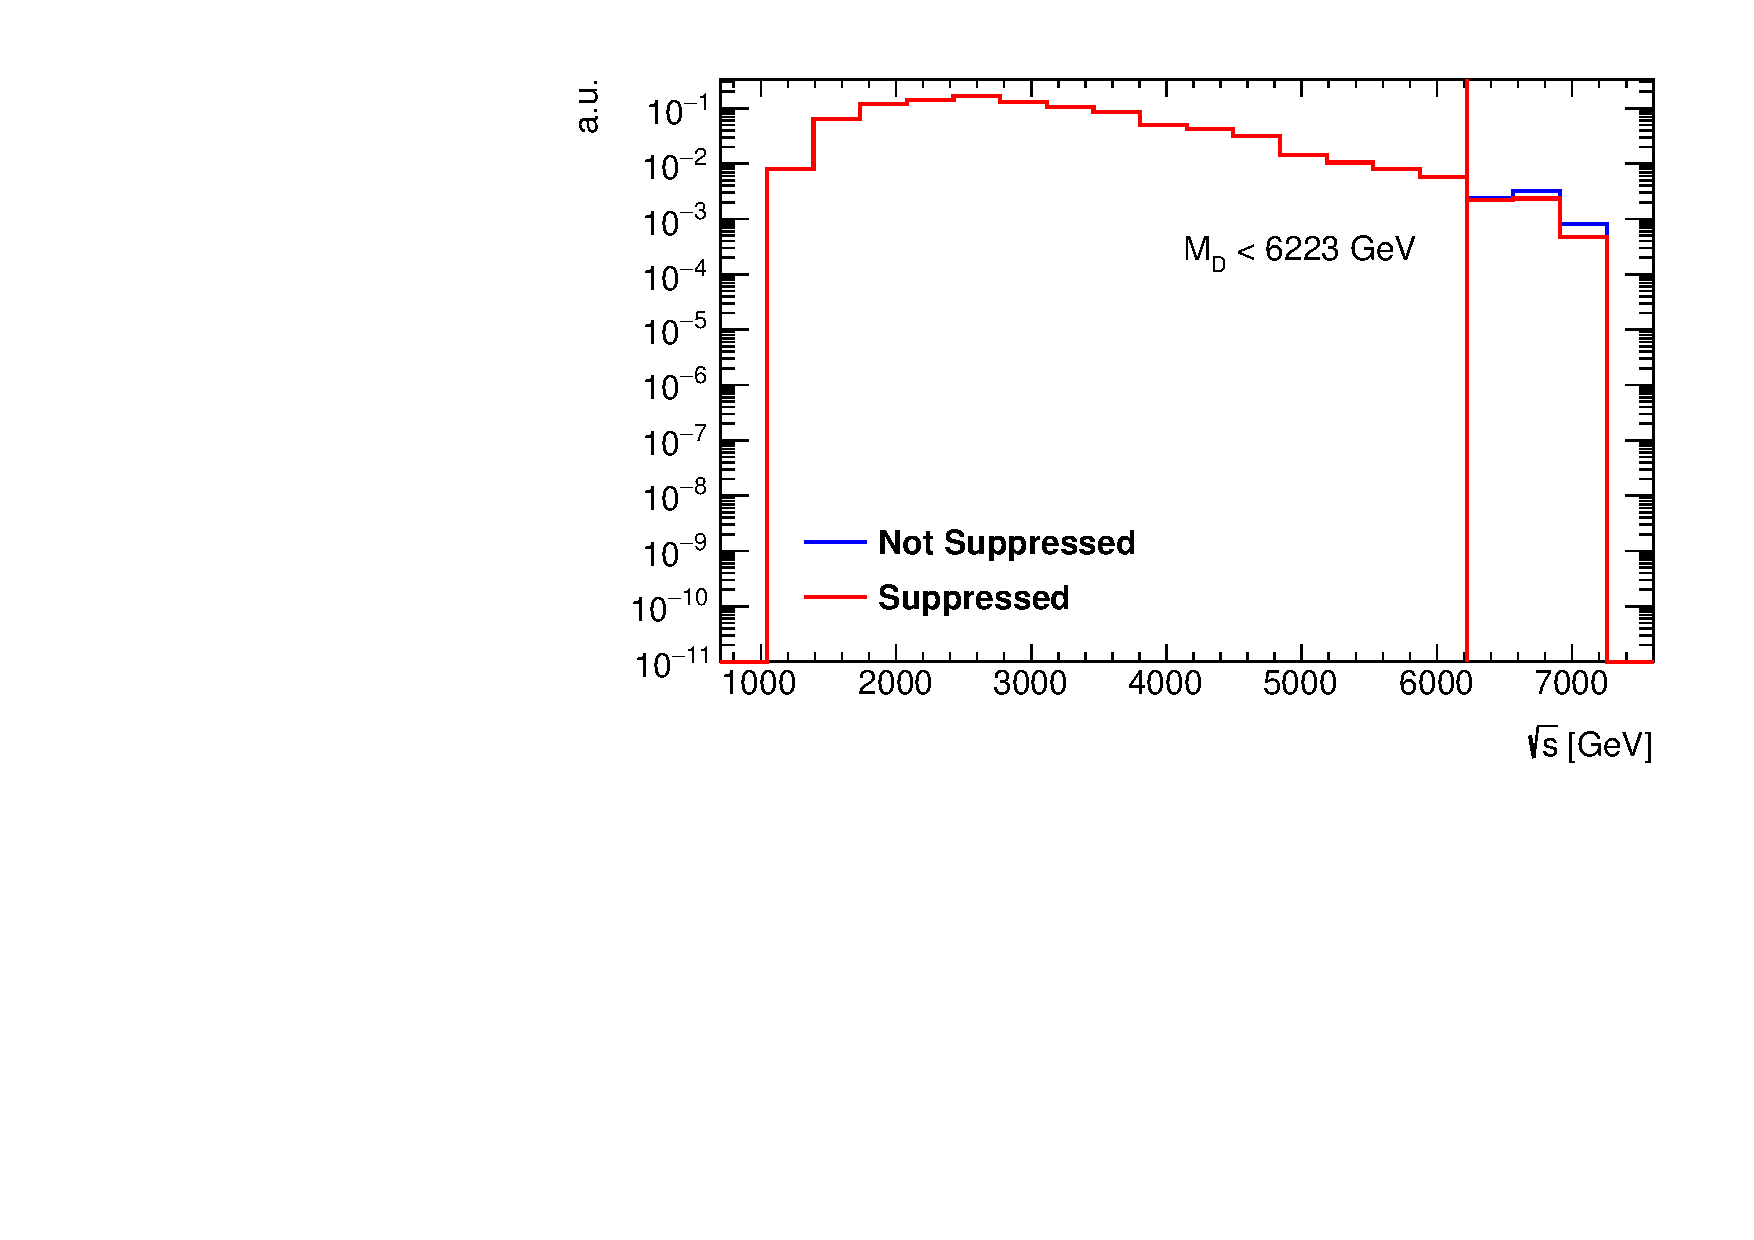
\includegraphics[width=\linewidth]{plot_nD3_SR700}
    \caption{ADD n = 3 for high $\met$ region.}
    \label{fig:shat_n3_700}
  \end{subfigure}
  \begin{subfigure}{.48\linewidth}
    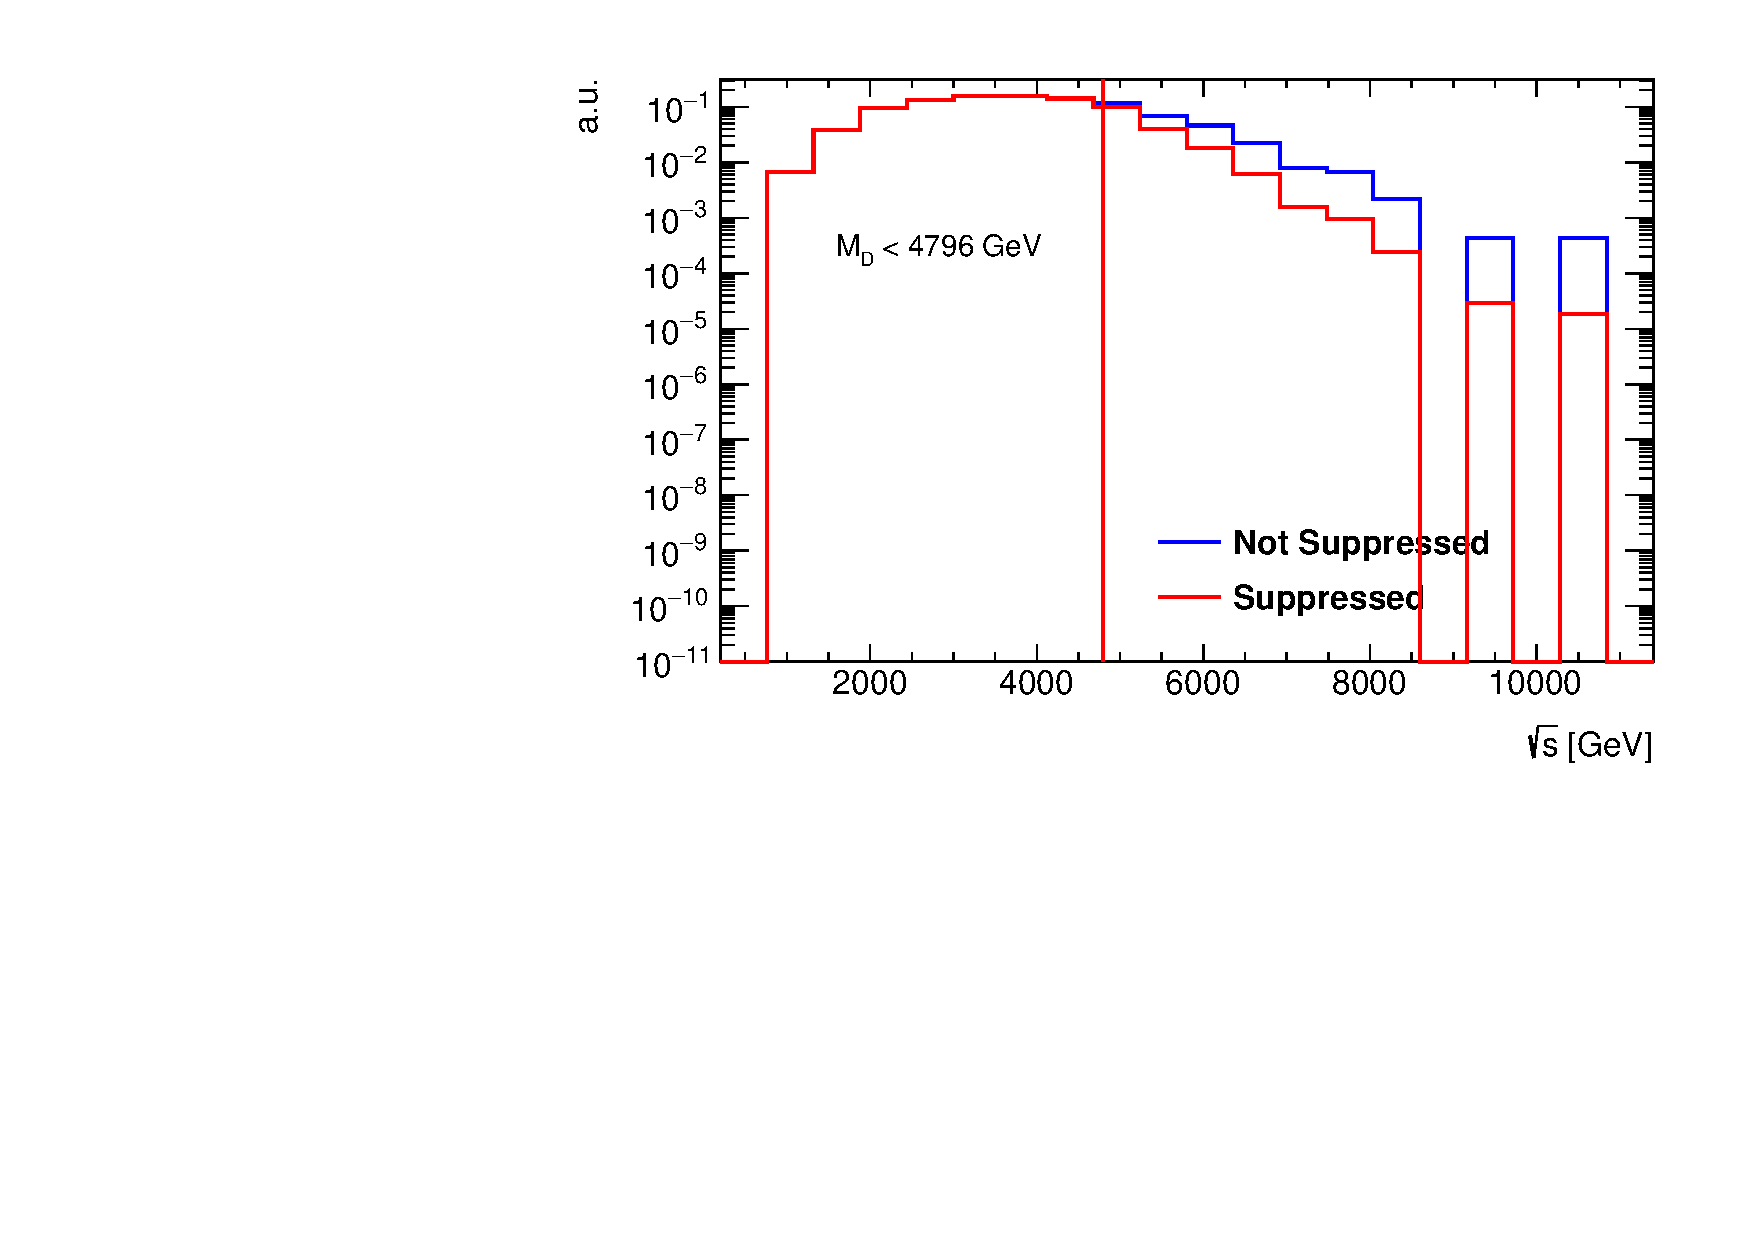
\includegraphics[width=\linewidth]{plot_nD6_SR250}
    \caption{ADD n = 6 for low $\met$ region.}
    \label{fig:shat_n6_250}
  \end{subfigure}
  \begin{subfigure}{.48\linewidth}
    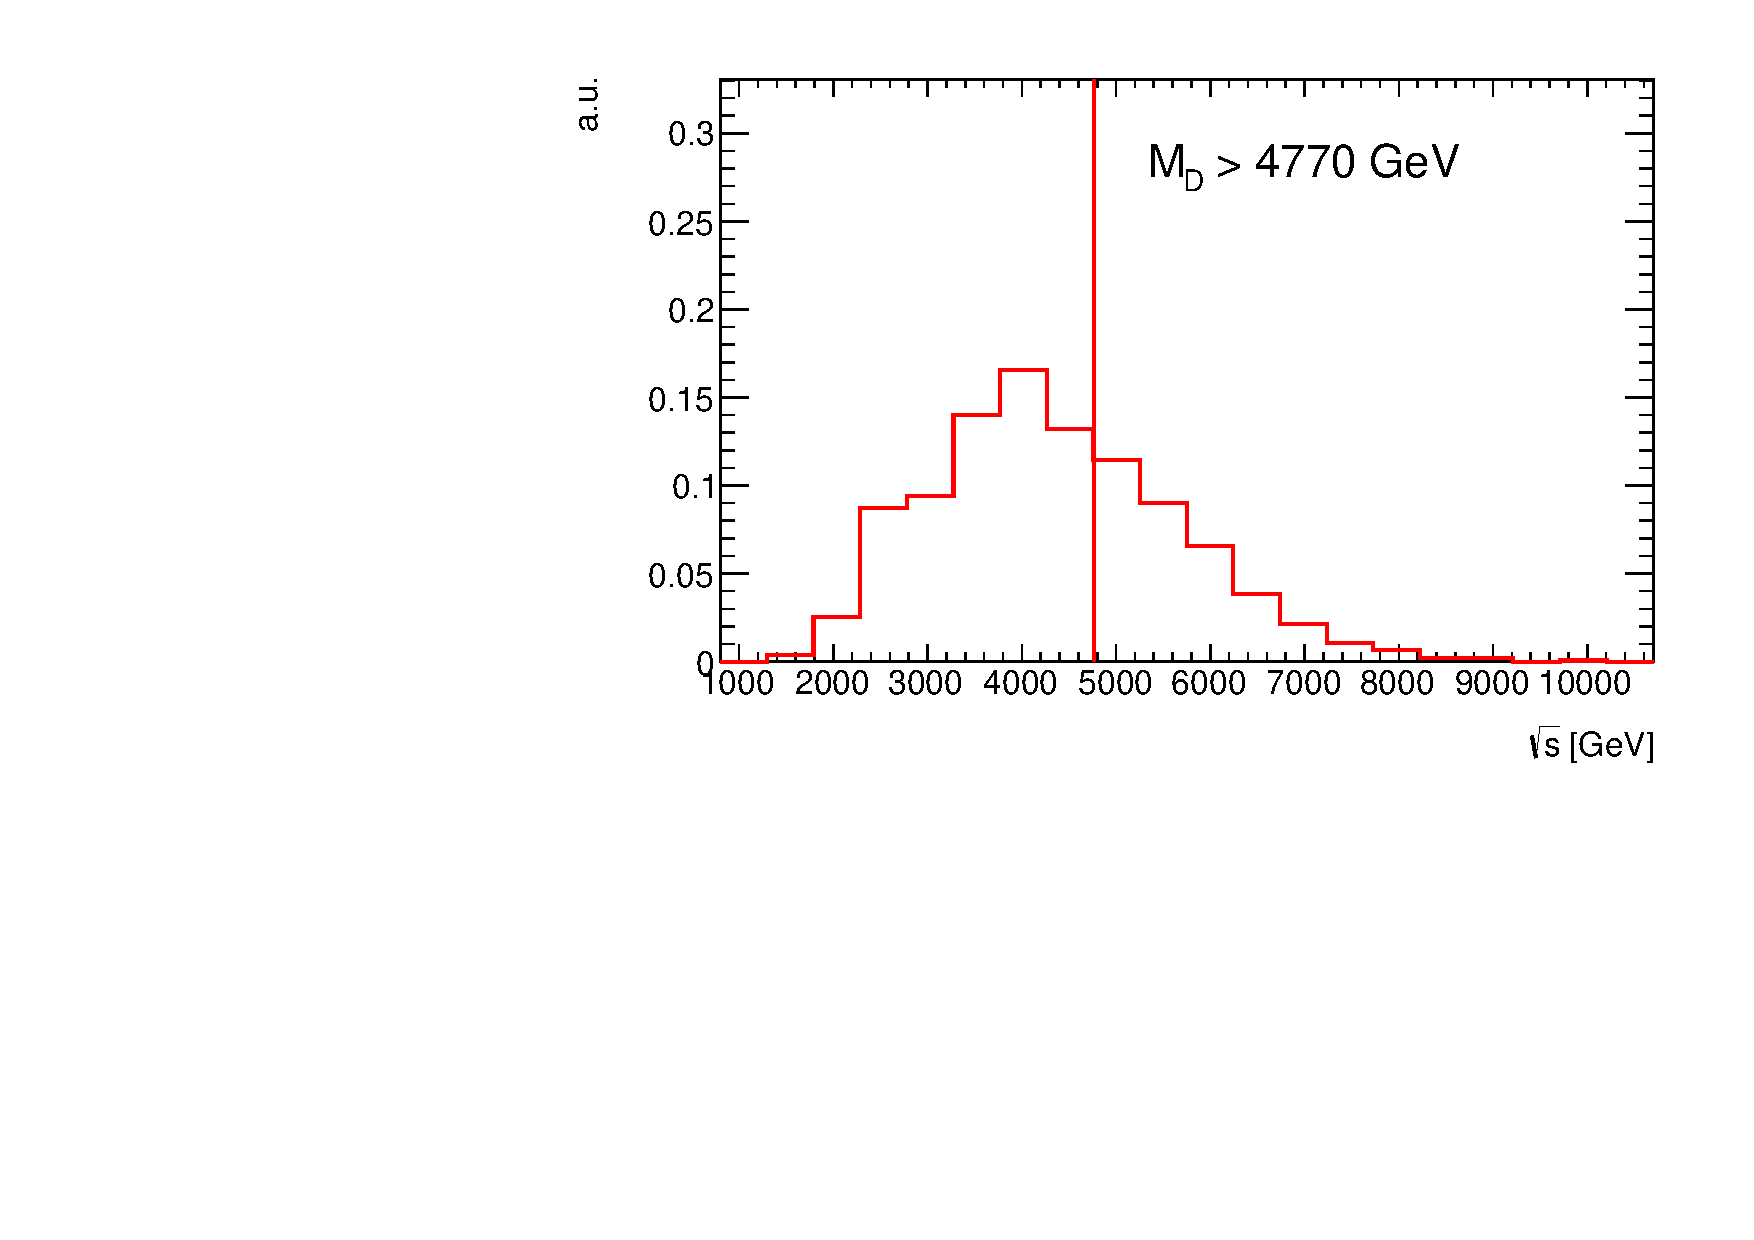
\includegraphics[width=\linewidth]{plot_nD6_SR700}
    \caption{ADD n = 6 for high $\met$ region.}
    \label{fig:shat_n6_700}
  \end{subfigure}
  \caption{Generated $\hat{s}$ distribution with and without weighting of the
    events for which $\hat{s} > \md^2$ for the signal regions where
    $250 < \met < 300$~GeV and $700 < \met < 800$~GeV for the ADD n = 3 and 6
    models for the 13~TeV \gls{mc}. A vertical line indicating the value of the
    excluded value of $\md$ is also reported in the figure.}
  \label{fig:shat}
\end{figure}
\begin{figure}[!h]
  \centering
  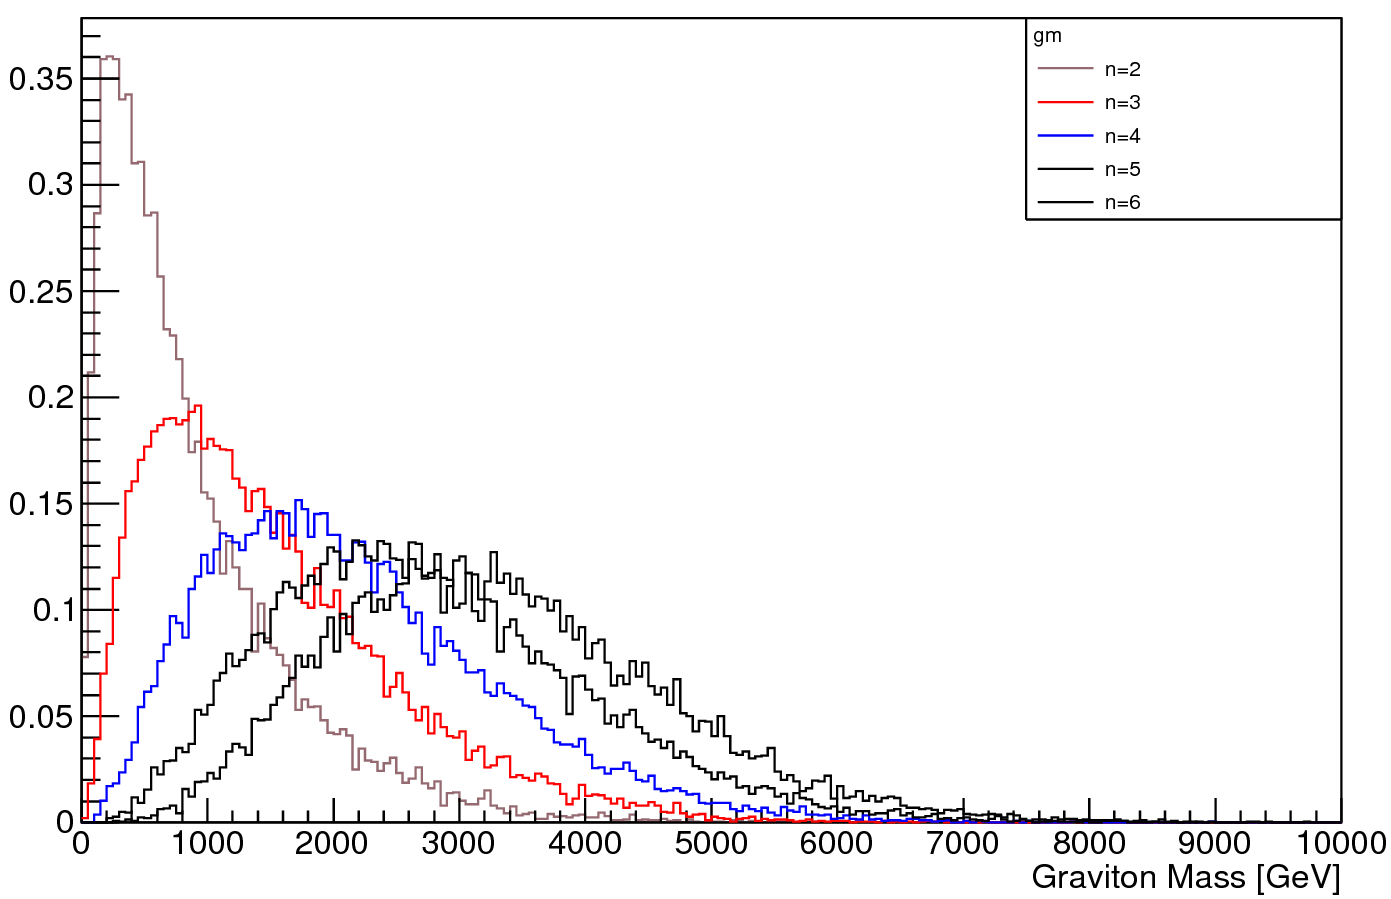
\includegraphics[width=.8\linewidth]{graviton_mass}
  \caption{Simulated graviton masses for the five different simulated extra
    dimensions.}
  \label{fig:graviton_mass}
\end{figure}
\begin{figure}[!h]
  \centering
  \begin{subfigure}{.48\linewidth}
    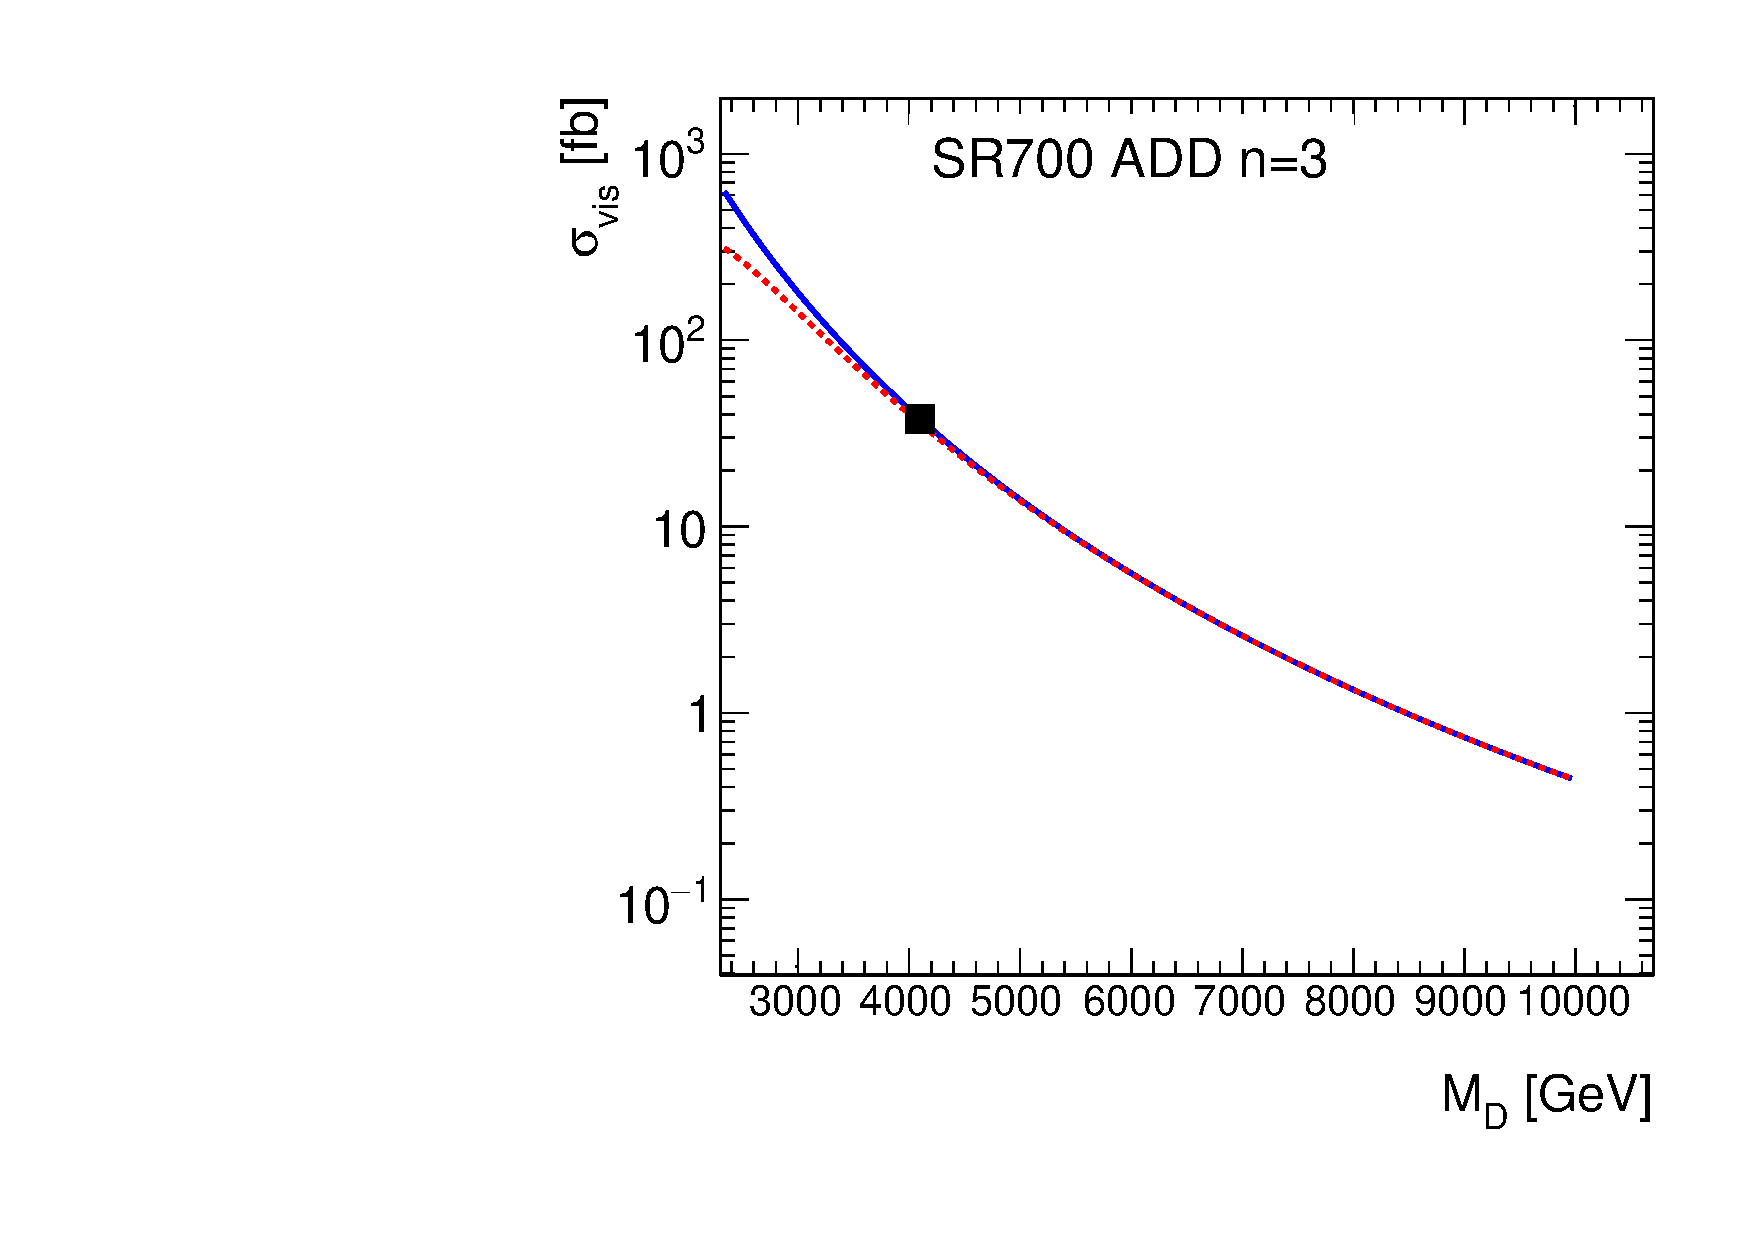
\includegraphics[width=\linewidth]{plot_sigma_visible_nD3_SR700}
    \caption{}
    \label{fig:sigma_vis_n3}
  \end{subfigure}
  \begin{subfigure}{.48\linewidth}
    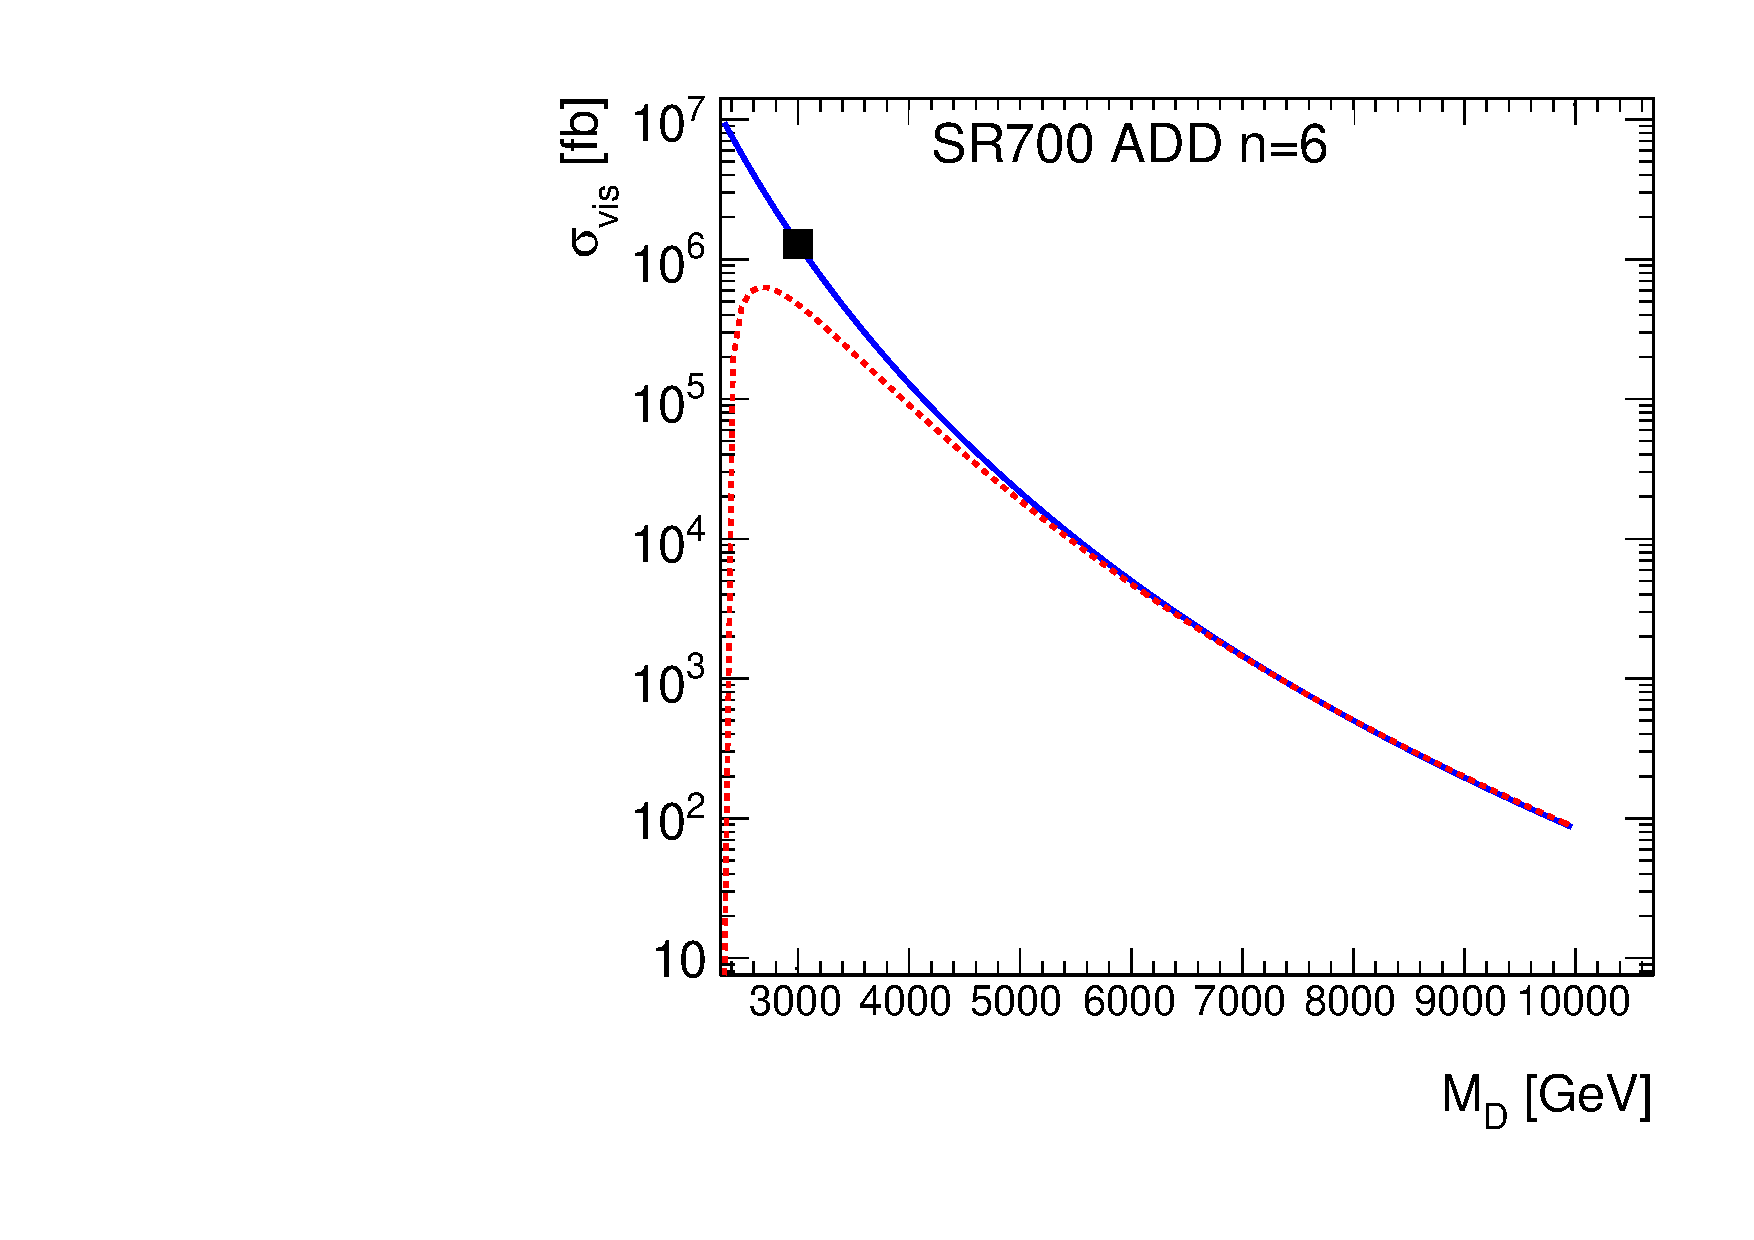
\includegraphics[width=\linewidth]{plot_sigma_visible_nD6_SR700}
    \caption{}
    \label{fig:sigma_vis_n6}
  \end{subfigure}
  \caption{Visible cross section as a function of $\md$ for the signal region
    where $250 < \met < 300$~GeV and $700 < \met < 800$~GeV for the ADD n = 3
    and 6 models. The solid line is the visible cross section for all the
    $\hat{s}$, while in the dashed one a $\md^4/\hat{s}^2$ weighting factor is
    applied for events where $\hat{s} > \md^2$. The black square is the nominal
    $\md$ value of the generated sample.}
  \label{fig:vis_sigma_trunc}
\end{figure}
%%% Local Variables:
%%% mode: latex
%%% TeX-master: "../search_for_DM_LED_with_ATLAS"
%%% End:
